\documentclass[a4paper,12pt, unknownkeysallowed]{extreport}
\usepackage{cmap} % Улучшенный поиск русских слов в полученном pdf-файле
\usepackage[T2A]{fontenc} % Поддержка русских букв
\usepackage[utf8]{inputenc} % Кодировка utf8
\usepackage[english,russian]{babel} % Языки: русский, английский
%\usepackage{pscyr} % Нормальные шрифты
\usepackage{enumitem}

\usepackage[normalem]{ulem}
\usepackage{cancel}
\usepackage{float}
\usepackage[14pt]{extsizes}

\usepackage{caption}
\captionsetup{labelsep=endash}
\captionsetup[figure]{name={Рисунок}}

\usepackage{amsmath}

\usepackage{geometry}
\geometry{left=30mm}
\geometry{right=15mm}
\geometry{top=20mm}
\geometry{bottom=20mm}

\usepackage{titlesec}
\titleformat{\section}
	{\normalsize\bfseries}
	{\thesection}
	{1em}{}
\titlespacing*{\chapter}{0pt}{-30pt}{8pt}
\titlespacing*{\section}{\parindent}{*4}{*4}
\titlespacing*{\subsection}{\parindent}{*4}{*4}

\usepackage{setspace}
\onehalfspacing % Полуторный интервал

\frenchspacing
\usepackage{indentfirst} % Красная строка

\usepackage{titlesec}
\titleformat{\chapter}{\LARGE\bfseries}{\thechapter}{20pt}{\LARGE\bfseries}
\titleformat{\section}{\Large\bfseries}{\thesection}{20pt}{\Large\bfseries}

\usepackage{listings}
\usepackage{xcolor}

% Для листинга кода:
\lstset{ %
	language=c++,   					% выбор языка для подсветки	
	basicstyle=\small\sffamily,			% размер и начертание шрифта для подсветки кода
	numbers=left,						% где поставить нумерацию строк (слева\справа)
	%numberstyle=,					% размер шрифта для номеров строк
	stepnumber=1,						% размер шага между двумя номерами строк
	numbersep=5pt,						% как далеко отстоят номера строк от подсвечиваемого кода
	frame=single,						% рисовать рамку вокруг кода
	tabsize=4,							% размер табуляции по умолчанию равен 4 пробелам
	captionpos=t,						% позиция заголовка вверху [t] или внизу [b]
	breaklines=true,					
	breakatwhitespace=true,				% переносить строки только если есть пробел
	escapeinside={\#*}{*)},				% если нужно добавить комментарии в коде
	backgroundcolor=\color{white},
}

\usepackage{pgfplots}
\usetikzlibrary{datavisualization}
\usetikzlibrary{datavisualization.formats.functions}

\usepackage{graphicx}
\newcommand{\img}[3] {
	\begin{figure}[h!]
		\center{\includegraphics[height=#1]{inc/img/#2}}
		\caption{#3}
		\label{img:#2}
	\end{figure}
}
\newcommand{\boximg}[3] {
	\begin{figure}[h]
		\center{\fbox{\includegraphics[height=#1]{inc/img/#2}}}
		\caption{#3}
		\label{img:#2}
	\end{figure}
}

\usepackage[justification=centering]{caption} % Настройка подписей float объектов

\usepackage[unicode,pdftex]{hyperref} % Ссылки в pdf
\hypersetup{hidelinks}

\usepackage{csvsimple}

\setlength{\parindent}{1.25cm}

\makeatletter
\renewcommand\@biblabel[1]{#1.}
\makeatother

\newcommand{\code}[1]{\texttt{#1}}

\begin{document}

\begin{titlepage}
	\newgeometry{pdftex, left=2cm, right=2cm, top=2.5cm, bottom=2.5cm}
	\fontsize{12pt}{12pt}\selectfont
	\noindent \begin{minipage}{0.15\textwidth}
		
\includegraphics[width=\linewidth]{pictures/b_logo.jpg}
	\end{minipage}
	\noindent\begin{minipage}{0.9\textwidth}\centering
		\textbf{Министерство науки и высшего образования Российской Федерации}\\
		\textbf{Федеральное государственное бюджетное образовательное учреждение высшего образования}\\
		\textbf{«Московский государственный технический университет имени Н.Э.~Баумана}\\
		\textbf{(национальный исследовательский университет)»}\\
		\textbf{(МГТУ им. Н.Э.~Баумана)}
	\end{minipage}
	
	\noindent\rule{18cm}{3pt}
	\newline\newline
	\noindent ФАКУЛЬТЕТ $\underline{\text{«Информатика и системы управления»}}$ \newline\newline
	\noindent КАФЕДРА $\underline{\text{«Программное обеспечение ЭВМ и информационные технологии»}}$\newline\newline\newline\newline\newline\newline\newline
	
	
	\begin{center}
		\Large\textbf{Отчет по лабораторной работе №4}\newline
	\end{center}
	
	\noindent\textbf{Название} $\underline{\text{~Моделирование системы массового обслуживания~~~~~~~~~}}$\newline\newline\newline
	\noindent\textbf{Дисциплина} $\underline{\text{~Моделирование~~~~~~~~}}$\newline\newline
	\noindent\textbf{Студент} $\underline{\text{Золотухин А. В.~~~~~~~~~~~~~~~~~~~~~~~~~~~~~~~~~~~~~~~~~}}$\newline\newline
	\noindent\textbf{Группа} $\underline{\text{ИУ7-74Б~~~~~~~~~~~~~~~~~~~~~~~~~~~~~~~~~~~~~~~~~~~~}}$\newline\newline
	\noindent\textbf{Оценка (баллы)} $\underline{\text{~~~~~~~~~~~~~~~~~~~~~~~~~~~~~~~~~~~~~~~~~~~~~~~~~}}$\newline\newline
	\noindent\textbf{Преподаватель}$\underline{\text{~Рудаков И. В.~~~~~~~~~~}}$\newline
	
	\begin{center}
		\vfill
		Москва~---~\the\year
		~г.
	\end{center}
 \restoregeometry
\end{titlepage}


\chapter{Задание}

\section{Цель работы}

\textbf{Цель работы:} изучение венгерского метода решения задачи о назначениях.

\textbf{Задание:}
\begin{enumerate}
	\item Реализовать венгерский метод решения задачи о назначениях в виде программы на ЭВМ.
	\item Провести решение задачи с матрицей стоимостей, заданной в индивидуальном варианте, рассмотрев два случая:
	\begin{itemize}
		\item задача о назначениях является задачей минимизации,
		\item задача о назначениях является задачей максимизации.
	\end{itemize}
\end{enumerate}

\chapter{Теоретическая часть}

\section{Cодержательная и математическая постановки задачи о назначениях}

\textbf{Содержательная постановка:} имеется $n$ работ и $n$ исполнителей; стоимость выполнения $i$-ой работы $j$-ым исполнителем составляет $c_{ij} \geq 0$ единиц. Требуется распределить все работы между исполнителями так, чтобы
\begin{itemize}
	\item каждый исполнитель выполнял 1 работу;
	\item общая стоимость выполнения всех работ была $min$.
\end{itemize}

Введём управляемые переменные:
\begin{align}
	x_{ij} & =
	\begin{cases}
		1, \: \text{если $i$-ую работу выполняет $j$-ый работник}, \\
		0, \: \text{иначе};
	\end{cases} \nonumber \\
	i, j & = \overline{1; n}. 
\end{align}

Из переменных $x_{ij}$, $i,j = \overline{1; n}$, составим 
\begin{equation}
	X = (x_{ij}){, i,j = \overline{1; n}},
\end{equation}
которую назовём матрицей назначений.

Стоимости выполнения работ также записываем в матрицу
\begin{equation}
	C = (c_{ij}), {i,j = \overline{1; n}},
\end{equation}
называемой матрицей стоимостей.

Тогда:
\begin{enumerate}
	\item Стоимость выполнения работ:
	\begin{equation}
		f = \sum_{i=1}^n \sum_{j=1}^n c_{ij} x_{ij}.
	\end{equation}
	\item Условие того, что $i$-ую работу выполнит ровно один работник:
	\begin{equation}
		\sum_{j=1}^n x_{ij} = 1, \: i = \overline{1; n}.
	\end{equation}
	\item Условие того, что $j$-ый работник выполнит ровно одну работу:
	\begin{equation}
		\sum_{i=1}^n x_{ij} = 1, \: j = \overline{1; n}.
	\end{equation}
\end{enumerate}

Таким образом приходим к \textbf{математической постановке}:
\begin{equation}
	\begin{cases}
		f = \sum_{i=1}^n \sum_{j=1}^n c_{ij} x_{ij} \rightarrow min, \\
		\sum_{j=1}^n x_{ij} = 1, \: i = \overline{1; n}, \\
		\sum_{i=1}^n x_{ij} = 1, \: j = \overline{1; n}, \\
		x_{ij} \in \{0, 1\}, \: i,j = \overline{1; n}.
	\end{cases}
\end{equation}

\section{Исходные данные варианта №5}

\begin{equation}
	C = 
	\begin{bmatrix}
    9   &11&    3&    6&    6\\
	10   &9&   11&    5&    6\\
	8   &10&    5&    6&    4\\
	6    &8&   10&    4&    9\\
	11  &10&    9&    8&    7
	\end{bmatrix}
\end{equation}

\section{Краткое описание венгерского метода}

Схема венгерского метода решения задачи о назначениях представлена на рисунке \ref{fig:alg}.
\begin{figure}[H]
	\centering
	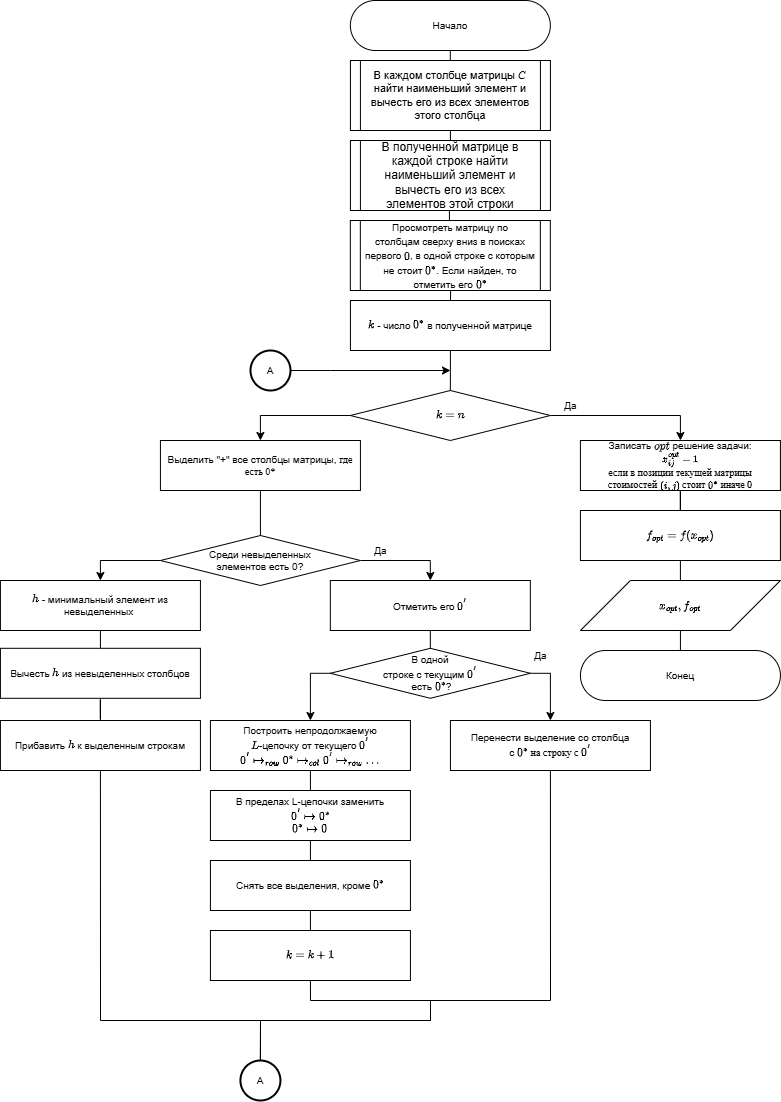
\includegraphics[width=1\linewidth]{alg}
	\caption[]{Схема венгерского метода}
	\label{fig:alg}
\end{figure}


\chapter{Практическая часть}


\begin{lstlisting}[language=Matlab]
function lab1()
	clc;
	debugMode = 1;
	findMax = 0;
	
	matr = [
	9   11    3    6    6;
	10   9   11    5    6;
	8   10    5    6    4;
	6    8   10    4    9;
	11  10    9    8    7];
	disp('5 вариант. Матрица:');
	disp(matr);
	
	C = matr;
	
	if findMax == 1
		C = convertToMin(matr);
	end
	
	if debugMode == 1
		disp('Матрица после приведения к задаче минимизации:');
		disp(C);
	end
	
	C = SubtractMinFromCols(C);
	if (debugMode == 1)
		disp('Вычесть минимум из каждого столбца');
		disp(C);
	end
	
	C = SubtractMinFromRows(C);
	if (debugMode == 1)
		disp('Вычесть минимум из каждой строки');
		disp(C);
	end
	
	snn = getSNN_Init(C);
	k = length(find(snn(:,2) > 0));
	if debugMode == 1
		disp('Начальная СНН');
		print_SNN(C, snn);
	end
	if debugMode == 1
		fprintf('Число нулей в построенной СНН: k = %d\n\n', k);
	end
	[r, c] = size(C);
	
	iteration = 1;
	while k < c
		if debugMode == 1
			fprintf('---------------- Итерация №%d ----------------\n', iteration);
		end
		
		shtrih = zeros(r * c / 2, 2);   % позиции 0'
		b = 1;
		selectedColumns = snn(:,2);
		selectedRows = zeros(1, r);
		selection = getSelection(r, c, selectedColumns);
		if debugMode == 1
			disp('Результат выделения столбцов, в которых стоит 0*:');
			printMarkedMatr(C, snn, shtrih, selectedColumns, selectedRows);
		end
		flag = true;
		shp = [-1 -1];
		while flag
			if debugMode == 1
				disp('Поиск 0 среди невыделенных элементов');
			end
			
			shp = findShtrih(C, selection);
			if shp(1) == -1
				C = updateMatrNoZero(C, r, c, selection, selectedRows, selectedColumns);
				if debugMode == 1
					disp('Т. к. среди невыделенных элементов нет нулей, матрица была преобразована:');
					printMarkedMatr(C, snn, shtrih, selectedColumns, selectedRows);
				end
				shp = findShtrih(C, selection);
			end
			
			shtrih(b,:) = shp;
			b = b+1;
			if debugMode == 1
				disp('Матрица с найденным 0- штрих');
				printMarkedMatr(C, snn, shtrih, selectedColumns, selectedRows);
			end
			
			zeroStarInRow = getZeroStarInRow(shp, snn);
			if isempty(zeroStarInRow)
				flag = false;
			else
				selection(:, zeroStarInRow(2)) = selection(:, zeroStarInRow(2)) - 1;
				selectedColumns(zeroStarInRow(2)) = 0;
				selection(zeroStarInRow(1), :) = selection(zeroStarInRow(1), :) + 1;
				selectedRows(zeroStarInRow(1)) = 1;
				if debugMode == 1
					disp('Т.к. в одной строке с 0- штрих есть 0*, было переброшено выделение:');
					printMarkedMatr(C, snn, shtrih, selectedColumns, selectedRows);
				end
			end
		end
		
		
		if debugMode == 1
			disp('L-цепочка: ');
		end
		
		[shtrih, snn] = createL(shp, shtrih, snn);
		
		k = length(find(snn(:,2) > 0));
		if debugMode == 1
			disp('Текущая СНН:');
			print_SNN(C, snn);
			fprintf('Итого, k = %d\n', k);
		end
		
		iteration = iteration + 1;
		disp('----------------------------------------------');
	end
	
	disp('Конечная СНН:');
	print_SNN(C, snn);
	
	disp('X =');
	print_X(snn);
	
	fOpt = getFOpt(matr, snn);
	fprintf("Результат = %d\n", fOpt);
end

function matr = convertToMin(matr)
	maxElem = max(matr, [], "all");
	matr = (-1) * matr + maxElem;
end

function matr = SubtractMinFromCols(matr)
	minElemArr = min(matr);
	for i = 1 : length(matr)
		matr(:, i) = matr(:, i) - minElemArr(i);
	end
end

function matr = SubtractMinFromRows(matr)
	minElemArr = min(matr, [], 2);
	for i = 1 : length(minElemArr)
		matr(i, :) = matr(i, :) - minElemArr(i);
	end
end

function SNN = getSNN_Init(matr)
	[m, n] = size(matr);
	SNN = zeros(n, 2);
	for i = 1: n
		for j = 1 : m
			if matr(j, i) == 0
				k = 1;
				while SNN(k, 1) ~= j && SNN(k, 2) ~= i && k < n
					k = k + 1;
				end
				if (k == n)
					SNN(i, 1) = j;
					SNN(i, 2) = i;
				end
			end
		end
	end
end

function [] = print_SNN(matr, SNN)
	[r, c] = size(matr);
	fprintf("\n");
	for i = 1 : r
		for j = 1 : c
			inds = [i, j];
			f = find(ismember(SNN,inds, "rows"), 1);
			if (f > 0) 
				fprintf("\t%d*", matr(i, j));
			else
				fprintf("\t%d", matr(i, j));
			end
		end
		fprintf("\n");
	end
	fprintf("\n");
end

function [] = print_X(SNN)
	[r, ~] = size(SNN);
	fprintf("\n");
	for i = 1 : r
		for j = 1 : r
			inds = [i, j];
			f = find(ismember(SNN,inds, "rows"), 1);
			if (f > 0) 
				fprintf("\t1");
			else
				fprintf("\t0");
			end
		end
		fprintf("\n");
	end
	fprintf("\n");
end

function [selection] = getSelection(r, c, selectedColumns)
	selection = zeros(r, c);
	for i = 1 : c
		if selectedColumns(i) > 0
			selection(:, i) = selection(:, i) + 1;
		end
	end
end

function [] = printMarkedMatr(matr, SNN, shtrih, selectedCols, selectedRows)
	[r,c] = size(matr);
	
	for i = 1 : r
		if selectedRows(i) > 0
			fprintf("+")
		end
		for j = 1 : c
			fprintf("\t%d", matr(i, j));
			inds = [i, j];
			f1 = find(ismember(SNN, inds, "rows"), 1);
			f2 = find(ismember(shtrih, inds, "rows"), 1);
			if (f1 > 0) 
				fprintf("*");
			elseif(f2 > 0)
				fprintf("'")
            end
        end
        fprintf('\n');
	end
	
	for i = 1 : c
		if selectedCols(i) > 0
			fprintf("\t+")
		else
			fprintf(" \t")
		end
	end
	fprintf('\n\n');
end

function [shp] = findShtrih(matr, selection)
	shp = [-1 -1];
	[r, c] = size(matr);
	for i = 1 : c
		for j = 1 : r
			if selection(j, i) == 0 && matr(j, i) == 0
				shp = [j, i];
				return;
			end
		end
	end
end

function [matr] = updateMatrNoZero(matr, r, c, selection, selectedRows, selectedColumns)
	h = 1e5;
	for i = 1 : c
		for j = 1 : r
			if selection(j, i) == 0 && matr(j, i) < h
				h = matr(j, i);
			end
		end
	end

	for i = 1 : c
		if selectedColumns(i) == 0
			matr(:, i) = matr(:, i) - h;
		end
	end
	for i = 1 : r
		if selectedRows(i) > 0
			matr(i, :) = matr(i, :) + h;
		end
	end
end

function [zeroStarInRow] = getZeroStarInRow(shp, snn)
	j = shp(1);
	i = snn(:,1)==j;
	zeroStarInRow = snn(i, :);
end

function [shtrih, snn] = createL(shp, shtrih, snn)
	i = shp(1);
	j = shp(2);
	fprintf("[%d, %d]\n", i, j);
	while true
		inds = [i, j];
		k = ismember(shtrih, inds, "rows");
		shtrih(k, :) = [0, 0];
		k = snn(:,2)==j;
		
		if k==0
			snn(j,:) = inds;
			break;
		end
		s = snn(k,:);
		fprintf("[%d, %d] -> ", s(1), s(2));
		snn(j,:) = inds;
		k = shtrih(:,1)==s(2);
		inds = shtrih(k,:);
		i = inds(1);
		j = inds(2);
		fprintf("[%d, %d]", i, j);
		fprintf("\n");
	end
end

function [fOpt] = getFOpt(matr, snn)
	fOpt = 0;
	[r,~] = size(snn);
	
	for i = 1 : r
		fOpt = fOpt + matr(snn(i, 1), snn(i, 2));
	end
end
\end{lstlisting}

\section{Результаты расчетов}

Решение задачи минимизации.

\begin{verbatim}
5 вариант. Матрица:
9     11     3     6     6
10     9    11     5     6
8     10     5     6     4
6      8    10     4     9
11    10     9     8     7

Матрица после приведения к задаче минимизации:
9     11     3     6     6
10     9    11     5     6
8     10     5     6     4
6      8    10     4     9
11    10     9     8     7

Вычесть минимум из каждого столбца
3     3     0     2     2
4     1     8     1     2
2     2     2     2     0
0     0     7     0     5
5     2     6     4     3





Вычесть минимум из каждой строки
3     3     0     2     2
3     0     7     0     1
2     2     2     2     0
0     0     7     0     5
3     0     4     2     1

Начальная СНН

3   3   0*  2   2
3   0*  7   0   1
2   2   2   2   0*
0*  0   7   0   5
3   0   4   2   1

Число нулей в построенной СНН: k = 4

---------------- Итерация №1 ----------------
Результат выделения столбцов, в которых стоит 0*:
3   3   0*  2   2
3   0*  7   0   1
2   2   2   2   0*
0*  0   7   0   5
3   0   4   2   1
+   +   +       +

Поиск 0 среди невыделенных элементов
Матрица с найденным 0-штрих
3   3   0*  2   2
3   0*  7   0'  1
2   2   2   2   0*
0*  0   7   0   5
3   0   4   2   1
+   +   +       +

Т.к. в одной строке с 0-штрих есть 0*, было переброшено выделение:
    3   3   0*  2   2
+   3   0*  7   0'   1
    2   2   2   2   0*
    0*  0   7   0   5
    3   0   4   2   1
    +       +       +

Поиск 0 среди невыделенных элементов
Матрица с найденным 0-штрих
    3   3   0*  2   2
+   3   0*  7   0'  1
    2   2   2   2   0*
    0*  0'  7   0   5
    3   0   4   2   1
    +       +       +

Т.к. в одной строке с 0-штрих есть 0*, было переброшено выделение:
    3   3   0*  2   2
+   3   0*  7   0'  1
    2   2   2   2   0*
+   0*  0'  7   0   5
    3   0   4   2   1
        +       +

Поиск 0 среди невыделенных элементов
Матрица с найденным 0-штрих
    3   3   0*  2   2
+   3   0*  7   0'  1
    2   2   2   2   0*
+   0*  0'  7   0   5
    3   0'  4   2   1
        +       +

L-цепочка: 
[5, 2]
[2, 2] -> [2, 4]
Текущая СНН:

3   3   0*  2   2
3   0   7   0*  1
2   2   2   2   0*
0*  0   7   0   5
3   0*  4   2   1

Итого, k = 5
----------------------------------------------
Конечная СНН:

3   3   0*  2   2
3   0   7   0*  1
2   2   2   2   0*
0*  0   7   0   5
3   0*  4   2   1

X =
0   0   1   0   0
0   0   0   1   0
0   0   0   0   1
1   0   0   0   0
0   1   0   0   0

Результат = 28
\end{verbatim}

Решение задачи максимизации.

\begin{verbatim}
5 вариант. Матрица:
9     11     3     6     6
10     9    11     5     6
8     10     5     6     4
6      8    10     4     9
11    10     9     8     7

Матрица после приведения к задаче минимизации:
2     0     8     5     5
1     2     0     6     5
3     1     6     5     7
5     3     1     7     2
0     1     2     3     4

Вычесть минимум из каждого столбца
2     0     8     2     3
1     2     0     3     3
3     1     6     2     5
5     3     1     4     0
0     1     2     0     2

Вычесть минимум из каждой строки
2     0     8     2     3
1     2     0     3     3
2     0     5     1     4
5     3     1     4     0
0     1     2     0     2

Начальная СНН

2   0*  8   2   3
1   2   0*  3   3
2   0   5   1   4
5   3   1   4   0*
0*  1   2   0   2

Число нулей в построенной СНН: k = 4

---------------- Итерация №1 ----------------
Результат выделения столбцов, в которых стоит 0*:
2   0*  8   2   3
1   2   0*  3   3
2   0   5   1   4
5   3   1   4   0*
0*  1   2   0   2
+   +   +       +

Поиск 0 среди невыделенных элементов
Матрица с найденным 0-штрих
2   0*  8   2   3
1   2   0*  3   3
2   0   5   1   4
5   3   1   4   0*
0*  1   2   0'  2
+   +   +       +

Т.к. в одной строке с 0-штрих есть 0*, было переброшено выделение:
    2   0*  8   2   3
    1   2   0*  3   3
    2   0   5   1   4
    5   3   1   4   0*
+   0*  1   2   0'  2
        +   +       +
        
        
        
        
        

Поиск 0 среди невыделенных элементов
Т.к. среди невыделенных элементов нет нулей, матрица была преобразована:
    1   0*  8   1   3
    0   2   0*  2   3
    1   0   5   0   4
    4   3   1   3   0*
+   0*  2   3   0'  3
        +   +       +

Матрица с найденным 0-штрих
    1   0*  8   1   3
    0'  2   0*  2   3
    1   0   5   0   4
    4   3   1   3   0*
+   0*  2   3   0'  3
        +   +       +

Т.к. в одной строке с 0-штрих есть 0*, было переброшено выделение:
    1   0*  8   1   3
+   0'  2   0*  2   3
    1   0   5   0   4
    4   3   1   3   0*
+   0*  2   3   0'  3
        +           +

Поиск 0 среди невыделенных элементов
Матрица с найденным 0-штрих
    1   0*  8   1   3
+   0'  2   0*  2   3
    1   0   5   0'  4
    4   3   1   3   0*
+   0*  2   3   0'  3
        +           +

L-цепочка: 
[3, 4]
Текущая СНН:

1   0*  8   1   3
0   2   0*  2   3
1   0   5   0*  4
4   3   1   3   0*
0*  2   3   0   3

Итого, k = 5
----------------------------------------------
Конечная СНН:

1   0*  8   1   3
0   2   0*  2   3
1   0   5   0*  4
4   3   1   3   0*
0*  2   3   0   3

X =
0   1   0   0   0
0   0   1   0   0
0   0   0   1   0
0   0   0   0   1
1   0   0   0   0

Результат = 48
\end{verbatim}

\end{document}
